\documentclass[12pt]{article}
\usepackage{tikz}
\usepackage{amsmath}
% Underlining package
\usepackage{ulem}
\usetikzlibrary{calc}
\usetikzlibrary{angles,quotes}
\usepackage[a4paper, portrait, margin=1cm]{geometry}
\usepackage{fancyhdr}

\newcommand{\HeadingAnswers}{%
\section*{\Large Name: \underline{\hspace{8cm}} \hfill Date: \underline{\hspace{3cm}}}%
\vspace{-3mm}\par
\textbf{Area Rectangles: Answers}\vspace{1pt}\hrule
}

% raise footer with page number; no header
\fancypagestyle{myfancypagestyle}{
  \fancyhf{}% clear all header and footer fields
  \renewcommand{\headrulewidth}{0pt} % no rule under header
  \fancyfoot[C] {\thepage} \setlength{\footskip}{14.5pt} % raise page number allowed min 14.5pt
}
\pagestyle{myfancypagestyle}  % apply myfancypagestyle

\newcounter{minipagecount}

\begin{document}
\HeadingAnswers
\vspace{8mm}

\begin{minipage}{0.55\textwidth}
  \refstepcounter{minipagecount}
  \noindent{(\theminipagecount)}\quad
 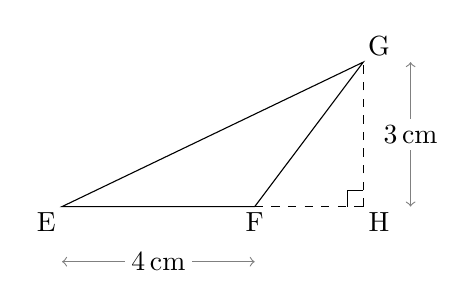
\begin{tikzpicture}[scale=1.0, baseline=(current bounding box.north)]
        \begin{scope}[rotate=0]

        \coordinate (E) at (0,0);
        \coordinate (F) at (2.447,0);
        \coordinate (H) at ($(F)+(1.379,0)$);  % extend out
        \coordinate (G) at ($(H)+(0,1.835)$); % Perpendicular upwards

        \draw (E)--(F)--(G)--cycle;
        \draw[dashed] (F)--(H);
        \draw[dashed] (H)--(G);
        \pic [draw, -, angle radius=0.2cm] {right angle=G--H--F};

        % Vertex LABELS
        % Labels relative to shape geometry
        \node at ($(E)+(-0.2,-0.2)$) {E};
        \node at ($(F)+(0.0,-0.2)$) {F};
        \node at ($(H)+(0.2,-0.2)$) {H};
        \node at ($(G)+(0.2,0.2)$) {G};


        % dotted/dashed arrows shifted away from edges
        % Horizontal side (A-B), shifted down yshift=0mm,
        \draw[<->, gray]
            ($(E) + (0,-0.7cm)$) -- ($(F) + (0,-0.7cm)$)
            node[black, midway, fill=white, inner sep=2.5pt] {4\,cm};

        % Vertical side (D-C), shifted right xshift=0mm,
        \draw[<->, gray]
            ($(H)+(0.6,0)$) -- ($(H |- G)+(0.6,0)$)
            node[black, midway, fill=white, inner sep=2.5pt] {3\,cm};
    \end{scope}
\end{tikzpicture}
\end{minipage}%
\hfill
\begin{minipage}{.4\textwidth}
  \begin{align*}
    \text{Area} &= \frac{1}{2} \text{bh} \\
    \text{Area} &= \frac{1}{2} \times 4 \text{cm} \times 3 \text{cm}  \\
    \text{Area} &= 6.0 \text{cm}^2
  \end{align*}
\end{minipage}

\par\vspace{1cm}\begin{minipage}{0.55\textwidth}
  \refstepcounter{minipagecount}
  \noindent{(\theminipagecount)}\quad
 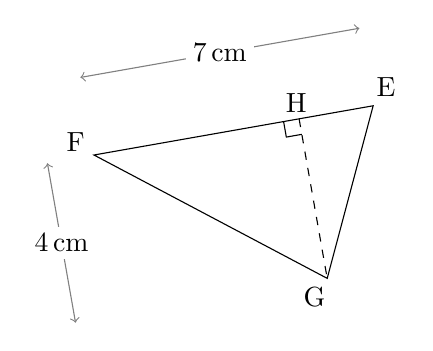
\begin{tikzpicture}[scale=1.0, baseline=(current bounding box.north)]
        \begin{scope}[rotate=190]

        \coordinate (E) at (0,0);
        \coordinate (F) at (3.6,0);
        \coordinate (H) at (0.955,0);
        \coordinate (G) at ($(H)+(0,2.057)$); % Perpendicular upwards

        \draw (E)--(F)--(G)--cycle;
        \draw[dashed] (H)--(G);
        \pic [draw, -, angle radius=0.2cm] {right angle=G--H--F};

        % Vertex LABELS
        % Labels relative to shape geometry
        \node at ($(E)+(-0.2,-0.2)$) {E};
        \node at ($(F)+(0.2,-0.2)$) {F};
        \node at ($(H)+(0.0,-0.2)$) {H};
        \node at ($(G)+(0.2,0.2)$) {G};


        % dotted/dashed arrows shifted away from edges
        % Horizontal side (A-B), shifted down  ift=0mm,
        \draw[<->, gray]
            ($(E) + (0,-1.0cm)$) -- ($(F) + (0,-1.0cm)$)
            node[black, midway, fill=white, inner sep=2.5pt] {7\,cm};

        % Vertical side (B-C), shifted right xshift=0mm,
        \draw[<->, gray]
            ($(F |- H)+(0.6,0)$) -- ($(F |- G)+(0.6,0)$)
            node[black, midway, fill=white, inner sep=2.5pt] {4\,cm};

    \end{scope}
\end{tikzpicture}
\end{minipage}%
\hfill
\begin{minipage}{.4\textwidth}
  \begin{align*}
    \text{Area} &= \frac{1}{2} \text{bh} \\
    \text{Area} &= \frac{1}{2} \times 7 \text{cm} \times 4 \text{cm}  \\
    \text{Area} &= 14.0 \text{cm}^2
  \end{align*}
\end{minipage}

\par\vspace{1cm}\begin{minipage}{0.55\textwidth}
  \refstepcounter{minipagecount}
  \noindent{(\theminipagecount)}\quad
 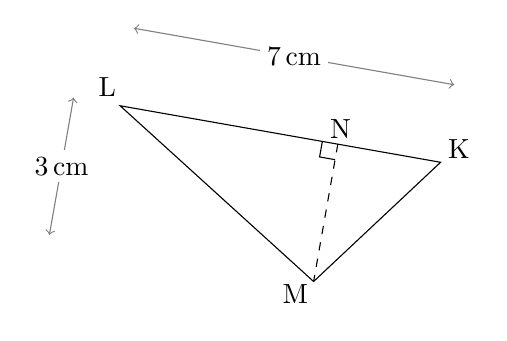
\begin{tikzpicture}[scale=1.0, baseline=(current bounding box.north)]
        \begin{scope}[rotate=170]

        \coordinate (K) at (0,0);
        \coordinate (L) at (4.132,0);
        \coordinate (N) at (1.325,0);
        \coordinate (M) at ($(N)+(0,1.771)$); % Perpendicular upwards

        \draw (K)--(L)--(M)--cycle;
        \draw[dashed] (N)--(M);
        \pic [draw, -, angle radius=0.2cm] {right angle=M--N--L};

        % Vertex LABELS
        % Labels relative to shape geometry
        \node at ($(K)+(-0.2,-0.2)$) {K};
        \node at ($(L)+(0.2,-0.2)$) {L};
        \node at ($(N)+(0.0,-0.2)$) {N};
        \node at ($(M)+(0.2,0.2)$) {M};


        % dotted/dashed arrows shifted away from edges
        % Horizontal side (A-B), shifted down  ift=0mm,
        \draw[<->, gray]
            ($(K) + (0,-1.0cm)$) -- ($(L) + (0,-1.0cm)$)
            node[black, midway, fill=white, inner sep=2.5pt] {7\,cm};

        % Vertical side (B-C), shifted right xshift=0mm,
        \draw[<->, gray]
            ($(L |- N)+(0.6,0)$) -- ($(L |- M)+(0.6,0)$)
            node[black, midway, fill=white, inner sep=2.5pt] {3\,cm};

    \end{scope}
\end{tikzpicture}
\end{minipage}%
\hfill
\begin{minipage}{.4\textwidth}
  \begin{align*}
    \text{Area} &= \frac{1}{2} \text{bh} \\
    \text{Area} &= \frac{1}{2} \times 7 \text{cm} \times 3 \text{cm}  \\
    \text{Area} &= 10.5 \text{cm}^2
  \end{align*}
\end{minipage}

\par\vspace{1cm}\begin{minipage}{0.55\textwidth}
  \refstepcounter{minipagecount}
  \noindent{(\theminipagecount)}\quad
 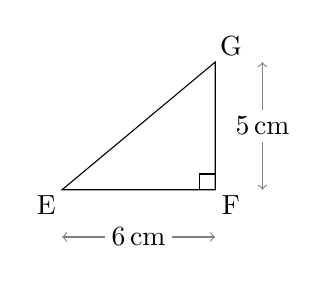
\begin{tikzpicture}[scale=1.0, baseline=(current bounding box.north)]
    \begin{scope}[rotate=0]
        % Draw

        \draw (0,0) coordinate (E) --
         ++(1.945,0) coordinate (F) --
         ++(90:1.621) coordinate (G) -- cycle;

        \pic [draw, -, angle radius=0.2cm] {right angle=G--F--E};

        % Vertex LABELS
        % Labels relative to shape geometry
        \node at ($(E)+(-0.2,-0.2)$) {E};
        \node at ($(F)+(0.2,-0.2)$) {F};
        \node at ($(G)+(0.2,0.2)$) {G};


        % dotted/dashed arrows shifted away from edges
        % Horizontal side (A-B), shifted down
        \draw[<->, gray]
            ($(E) + (0,-0.6cm)$) -- ($(F) + (0,-0.6cm)$)
            node[black, midway, fill=white, inner sep=2.5pt] {6\,cm};

        % Vertical side (B-C), shifted right
        \draw[<->, gray]
            ($(F) + (0.6cm,0)$) -- ($(G) + (0.6cm,0)$)
            node[black, midway, fill=white, xshift=0mm, inner sep=2.5pt] {5\,cm};

    \end{scope}
\end{tikzpicture}
\end{minipage}%
\hfill
\begin{minipage}{.4\textwidth}
  \begin{align*}
    \text{Area} &= \frac{1}{2} \text{bh} \\
    \text{Area} &= \frac{1}{2} \times 6 \text{cm} \times 5 \text{cm}  \\
    \text{Area} &= 15.0 \text{cm}^2
  \end{align*}
\end{minipage}

\par\vspace{1cm}\begin{minipage}{0.55\textwidth}
  \refstepcounter{minipagecount}
  \noindent{(\theminipagecount)}\quad
 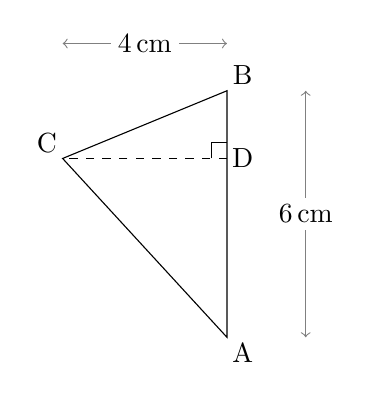
\begin{tikzpicture}[scale=1.0, baseline=(current bounding box.north)]
        \begin{scope}[rotate=90]

        \coordinate (A) at (0,0);
        \coordinate (B) at (3.131,0);
        \coordinate (D) at (2.271,0);
        \coordinate (C) at ($(D)+(0,2.087)$); % Perpendicular upwards

        \draw (A)--(B)--(C)--cycle;
        \draw[dashed] (D)--(C);
        \pic [draw, -, angle radius=0.2cm] {right angle=C--D--B};

        % Vertex LABELS
        % Labels relative to shape geometry
        \node at ($(A)+(-0.2,-0.2)$) {A};
        \node at ($(B)+(0.2,-0.2)$) {B};
        \node at ($(D)+(0.0,-0.2)$) {D};
        \node at ($(C)+(0.2,0.2)$) {C};


        % dotted/dashed arrows shifted away from edges
        % Horizontal side (A-B), shifted down  ift=0mm,
        \draw[<->, gray]
            ($(A) + (0,-1.0cm)$) -- ($(B) + (0,-1.0cm)$)
            node[black, midway, fill=white, inner sep=2.5pt] {6\,cm};

        % Vertical side (B-C), shifted right xshift=0mm,
        \draw[<->, gray]
            ($(B |- D)+(0.6,0)$) -- ($(B |- C)+(0.6,0)$)
            node[black, midway, fill=white, inner sep=2.5pt] {4\,cm};

    \end{scope}
\end{tikzpicture}
\end{minipage}%
\hfill
\begin{minipage}{.4\textwidth}
  \begin{align*}
    \text{Area} &= \frac{1}{2} \text{bh} \\
    \text{Area} &= \frac{1}{2} \times 6 \text{cm} \times 4 \text{cm}  \\
    \text{Area} &= 12.0 \text{cm}^2
  \end{align*}
\end{minipage}

\par\vspace{1cm}\begin{minipage}{0.55\textwidth}
  \refstepcounter{minipagecount}
  \noindent{(\theminipagecount)}\quad
 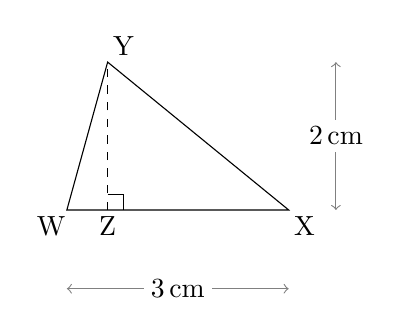
\begin{tikzpicture}[scale=1.0, baseline=(current bounding box.north)]
        \begin{scope}[rotate=0]

        \coordinate (W) at (0,0);
        \coordinate (X) at (2.817,0);
        \coordinate (Z) at (0.518,0);
        \coordinate (Y) at ($(Z)+(0,1.878)$); % Perpendicular upwards

        \draw (W)--(X)--(Y)--cycle;
        \draw[dashed] (Z)--(Y);
        \pic [draw, -, angle radius=0.2cm] {right angle=Y--Z--X};

        % Vertex LABELS
        % Labels relative to shape geometry
        \node at ($(W)+(-0.2,-0.2)$) {W};
        \node at ($(X)+(0.2,-0.2)$) {X};
        \node at ($(Z)+(0.0,-0.2)$) {Z};
        \node at ($(Y)+(0.2,0.2)$) {Y};


        % dotted/dashed arrows shifted away from edges
        % Horizontal side (A-B), shifted down  ift=0mm,
        \draw[<->, gray]
            ($(W) + (0,-1.0cm)$) -- ($(X) + (0,-1.0cm)$)
            node[black, midway, fill=white, inner sep=2.5pt] {3\,cm};

        % Vertical side (B-C), shifted right xshift=0mm,
        \draw[<->, gray]
            ($(X |- Z)+(0.6,0)$) -- ($(X |- Y)+(0.6,0)$)
            node[black, midway, fill=white, inner sep=2.5pt] {2\,cm};

    \end{scope}
\end{tikzpicture}
\end{minipage}%
\hfill
\begin{minipage}{.4\textwidth}
  \begin{align*}
    \text{Area} &= \frac{1}{2} \text{bh} \\
    \text{Area} &= \frac{1}{2} \times 3 \text{cm} \times 2 \text{cm}  \\
    \text{Area} &= 3.0 \text{cm}^2
  \end{align*}
\end{minipage}

\par\vspace{1cm}\begin{minipage}{0.55\textwidth}
  \refstepcounter{minipagecount}
  \noindent{(\theminipagecount)}\quad
 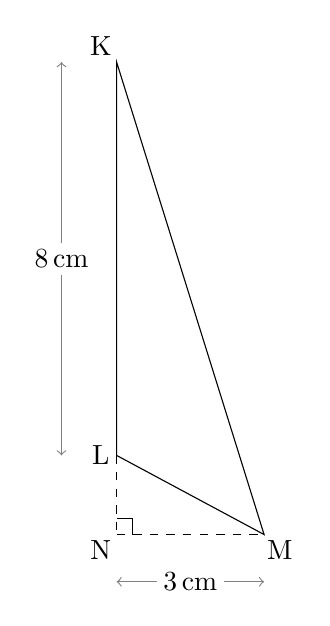
\begin{tikzpicture}[scale=1.0, baseline=(current bounding box.north)]
        \begin{scope}[rotate=270]

        \coordinate (K) at (0,0);
        \coordinate (L) at (4.995,0);
        \coordinate (N) at ($(L)+(1.005,0)$);  % extend out
        \coordinate (M) at ($(N)+(0,1.873)$); % Perpendicular upwards

        \draw (K)--(L)--(M)--cycle;
        \draw[dashed] (L)--(N);
        \draw[dashed] (N)--(M);
        \pic [draw, -, angle radius=0.2cm] {right angle=M--N--L};

        % Vertex LABELS
        % Labels relative to shape geometry
        \node at ($(K)+(-0.2,-0.2)$) {K};
        \node at ($(L)+(0.0,-0.2)$) {L};
        \node at ($(N)+(0.2,-0.2)$) {N};
        \node at ($(M)+(0.2,0.2)$) {M};


        % dotted/dashed arrows shifted away from edges
        % Horizontal side (A-B), shifted down yshift=0mm,
        \draw[<->, gray]
            ($(K) + (0,-0.7cm)$) -- ($(L) + (0,-0.7cm)$)
            node[black, midway, fill=white, inner sep=2.5pt] {8\,cm};

        % Vertical side (D-C), shifted right xshift=0mm,
        \draw[<->, gray]
            ($(N)+(0.6,0)$) -- ($(N |- M)+(0.6,0)$)
            node[black, midway, fill=white, inner sep=2.5pt] {3\,cm};
    \end{scope}
\end{tikzpicture}
\end{minipage}%
\hfill
\begin{minipage}{.4\textwidth}
  \begin{align*}
    \text{Area} &= \frac{1}{2} \text{bh} \\
    \text{Area} &= \frac{1}{2} \times 8 \text{cm} \times 3 \text{cm}  \\
    \text{Area} &= 12.0 \text{cm}^2
  \end{align*}
\end{minipage}

\par\vspace{1cm}\begin{minipage}{0.55\textwidth}
  \refstepcounter{minipagecount}
  \noindent{(\theminipagecount)}\quad
 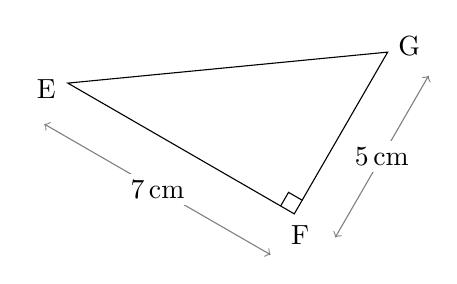
\begin{tikzpicture}[scale=1.0, baseline=(current bounding box.north)]
    \begin{scope}[rotate=-30]
        % Draw

        \draw (0,0) coordinate (E) --
         ++(3.321,0) coordinate (F) --
         ++(90:2.372) coordinate (G) -- cycle;

        \pic [draw, -, angle radius=0.2cm] {right angle=G--F--E};

        % Vertex LABELS
        % Labels relative to shape geometry
        \node at ($(E)+(-0.2,-0.2)$) {E};
        \node at ($(F)+(0.2,-0.2)$) {F};
        \node at ($(G)+(0.2,0.2)$) {G};


        % dotted/dashed arrows shifted away from edges
        % Horizontal side (A-B), shifted down
        \draw[<->, gray]
            ($(E) + (0,-0.6cm)$) -- ($(F) + (0,-0.6cm)$)
            node[black, midway, fill=white, inner sep=2.5pt] {7\,cm};

        % Vertical side (B-C), shifted right
        \draw[<->, gray]
            ($(F) + (0.6cm,0)$) -- ($(G) + (0.6cm,0)$)
            node[black, midway, fill=white, xshift=0mm, inner sep=2.5pt] {5\,cm};

    \end{scope}
\end{tikzpicture}
\end{minipage}%
\hfill
\begin{minipage}{.4\textwidth}
  \begin{align*}
    \text{Area} &= \frac{1}{2} \text{bh} \\
    \text{Area} &= \frac{1}{2} \times 7 \text{cm} \times 5 \text{cm}  \\
    \text{Area} &= 17.5 \text{cm}^2
  \end{align*}
\end{minipage}

\par\vspace{1cm}\begin{minipage}{0.55\textwidth}
  \refstepcounter{minipagecount}
  \noindent{(\theminipagecount)}\quad
 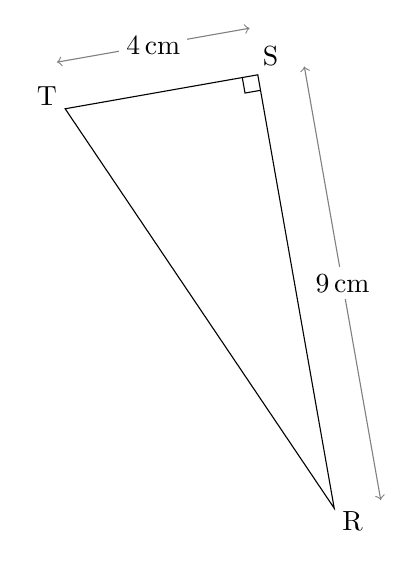
\begin{tikzpicture}[scale=1.0, baseline=(current bounding box.north)]
    \begin{scope}[rotate=100]
        % Draw

        \draw (0,0) coordinate (R) --
         ++(5.589,0) coordinate (S) --
         ++(90:2.484) coordinate (T) -- cycle;

        \pic [draw, -, angle radius=0.2cm] {right angle=T--S--R};

        % Vertex LABELS
        % Labels relative to shape geometry
        \node at ($(R)+(-0.2,-0.2)$) {R};
        \node at ($(S)+(0.2,-0.2)$) {S};
        \node at ($(T)+(0.2,0.2)$) {T};


        % dotted/dashed arrows shifted away from edges
        % Horizontal side (A-B), shifted down
        \draw[<->, gray]
            ($(R) + (0,-0.6cm)$) -- ($(S) + (0,-0.6cm)$)
            node[black, midway, fill=white, inner sep=2.5pt] {9\,cm};

        % Vertical side (B-C), shifted right
        \draw[<->, gray]
            ($(S) + (0.6cm,0)$) -- ($(T) + (0.6cm,0)$)
            node[black, midway, fill=white, xshift=0mm, inner sep=2.5pt] {4\,cm};

    \end{scope}
\end{tikzpicture}
\end{minipage}%
\hfill
\begin{minipage}{.4\textwidth}
  \begin{align*}
    \text{Area} &= \frac{1}{2} \text{bh} \\
    \text{Area} &= \frac{1}{2} \times 9 \text{cm} \times 4 \text{cm}  \\
    \text{Area} &= 18.0 \text{cm}^2
  \end{align*}
\end{minipage}

\par\vspace{1cm}\begin{minipage}{0.55\textwidth}
  \refstepcounter{minipagecount}
  \noindent{(\theminipagecount)}\quad
 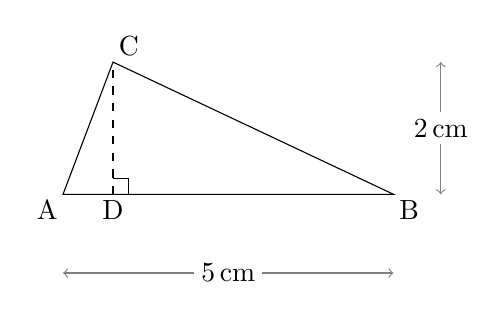
\begin{tikzpicture}[scale=1.0, baseline=(current bounding box.north)]
        \begin{scope}[rotate=0]

        \coordinate (A) at (0,0);
        \coordinate (B) at (4.197,0);
        \coordinate (D) at (0.635,0);
        \coordinate (C) at ($(D)+(0,1.679)$); % Perpendicular upwards

        \draw (A)--(B)--(C)--cycle;
        \draw[dashed] (D)--(C);
        \pic [draw, -, angle radius=0.2cm] {right angle=C--D--B};

        % Vertex LABELS
        % Labels relative to shape geometry
        \node at ($(A)+(-0.2,-0.2)$) {A};
        \node at ($(B)+(0.2,-0.2)$) {B};
        \node at ($(D)+(0.0,-0.2)$) {D};
        \node at ($(C)+(0.2,0.2)$) {C};


        % dotted/dashed arrows shifted away from edges
        % Horizontal side (A-B), shifted down  ift=0mm,
        \draw[<->, gray]
            ($(A) + (0,-1.0cm)$) -- ($(B) + (0,-1.0cm)$)
            node[black, midway, fill=white, inner sep=2.5pt] {5\,cm};

        % Vertical side (B-C), shifted right xshift=0mm,
        \draw[<->, gray]
            ($(B |- D)+(0.6,0)$) -- ($(B |- C)+(0.6,0)$)
            node[black, midway, fill=white, inner sep=2.5pt] {2\,cm};

    \end{scope}
\end{tikzpicture}
\end{minipage}%
\hfill
\begin{minipage}{.4\textwidth}
  \begin{align*}
    \text{Area} &= \frac{1}{2} \text{bh} \\
    \text{Area} &= \frac{1}{2} \times 5 \text{cm} \times 2 \text{cm}  \\
    \text{Area} &= 5.0 \text{cm}^2
  \end{align*}
\end{minipage}

\par\vspace{1cm}\begin{minipage}{0.55\textwidth}
  \refstepcounter{minipagecount}
  \noindent{(\theminipagecount)}\quad
 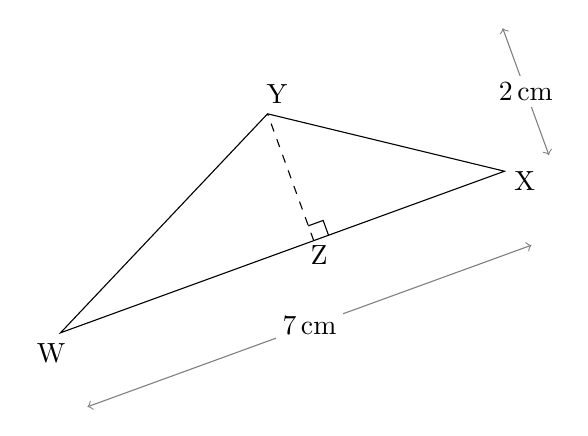
\begin{tikzpicture}[scale=1.0, baseline=(current bounding box.north)]
        \begin{scope}[rotate=20]

        \coordinate (W) at (0,0);
        \coordinate (X) at (6.0,0);
        \coordinate (Z) at (3.422,0);
        \coordinate (Y) at ($(Z)+(0,1.714)$); % Perpendicular upwards

        \draw (W)--(X)--(Y)--cycle;
        \draw[dashed] (Z)--(Y);
        \pic [draw, -, angle radius=0.2cm] {right angle=Y--Z--X};

        % Vertex LABELS
        % Labels relative to shape geometry
        \node at ($(W)+(-0.2,-0.2)$) {W};
        \node at ($(X)+(0.2,-0.2)$) {X};
        \node at ($(Z)+(0.0,-0.2)$) {Z};
        \node at ($(Y)+(0.2,0.2)$) {Y};


        % dotted/dashed arrows shifted away from edges
        % Horizontal side (A-B), shifted down  ift=0mm,
        \draw[<->, gray]
            ($(W) + (0,-1.0cm)$) -- ($(X) + (0,-1.0cm)$)
            node[black, midway, fill=white, inner sep=2.5pt] {7\,cm};

        % Vertical side (B-C), shifted right xshift=0mm,
        \draw[<->, gray]
            ($(X |- Z)+(0.6,0)$) -- ($(X |- Y)+(0.6,0)$)
            node[black, midway, fill=white, inner sep=2.5pt] {2\,cm};

    \end{scope}
\end{tikzpicture}
\end{minipage}%
\hfill
\begin{minipage}{.4\textwidth}
  \begin{align*}
    \text{Area} &= \frac{1}{2} \text{bh} \\
    \text{Area} &= \frac{1}{2} \times 7 \text{cm} \times 2 \text{cm}  \\
    \text{Area} &= 7.0 \text{cm}^2
  \end{align*}
\end{minipage}

\par\vspace{1cm}\begin{minipage}{0.55\textwidth}
  \refstepcounter{minipagecount}
  \noindent{(\theminipagecount)}\quad
 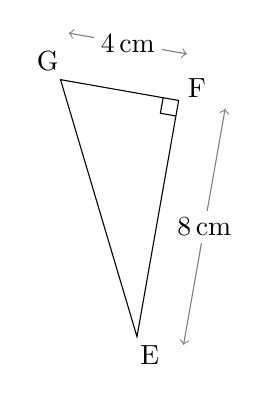
\begin{tikzpicture}[scale=1.0, baseline=(current bounding box.north)]
    \begin{scope}[rotate=80]
        % Draw

        \draw (0,0) coordinate (E) --
         ++(3.046,0) coordinate (F) --
         ++(90:1.523) coordinate (G) -- cycle;

        \pic [draw, -, angle radius=0.2cm] {right angle=G--F--E};

        % Vertex LABELS
        % Labels relative to shape geometry
        \node at ($(E)+(-0.2,-0.2)$) {E};
        \node at ($(F)+(0.2,-0.2)$) {F};
        \node at ($(G)+(0.2,0.2)$) {G};


        % dotted/dashed arrows shifted away from edges
        % Horizontal side (A-B), shifted down
        \draw[<->, gray]
            ($(E) + (0,-0.6cm)$) -- ($(F) + (0,-0.6cm)$)
            node[black, midway, fill=white, inner sep=2.5pt] {8\,cm};

        % Vertical side (B-C), shifted right
        \draw[<->, gray]
            ($(F) + (0.6cm,0)$) -- ($(G) + (0.6cm,0)$)
            node[black, midway, fill=white, xshift=0mm, inner sep=2.5pt] {4\,cm};

    \end{scope}
\end{tikzpicture}
\end{minipage}%
\hfill
\begin{minipage}{.4\textwidth}
  \begin{align*}
    \text{Area} &= \frac{1}{2} \text{bh} \\
    \text{Area} &= \frac{1}{2} \times 8 \text{cm} \times 4 \text{cm}  \\
    \text{Area} &= 16.0 \text{cm}^2
  \end{align*}
\end{minipage}

\par\vspace{1cm}\begin{minipage}{0.55\textwidth}
  \refstepcounter{minipagecount}
  \noindent{(\theminipagecount)}\quad
 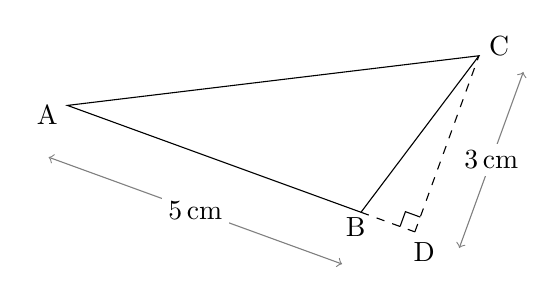
\begin{tikzpicture}[scale=1.0, baseline=(current bounding box.north)]
        \begin{scope}[rotate=-20]

        \coordinate (A) at (0,0);
        \coordinate (B) at (3.967,0);
        \coordinate (D) at ($(B)+(0.728,0)$);  % extend out
        \coordinate (C) at ($(D)+(0,2.38)$); % Perpendicular upwards

        \draw (A)--(B)--(C)--cycle;
        \draw[dashed] (B)--(D);
        \draw[dashed] (D)--(C);
        \pic [draw, -, angle radius=0.2cm] {right angle=C--D--B};

        % Vertex LABELS
        % Labels relative to shape geometry
        \node at ($(A)+(-0.2,-0.2)$) {A};
        \node at ($(B)+(0.0,-0.2)$) {B};
        \node at ($(D)+(0.2,-0.2)$) {D};
        \node at ($(C)+(0.2,0.2)$) {C};


        % dotted/dashed arrows shifted away from edges
        % Horizontal side (A-B), shifted down yshift=0mm,
        \draw[<->, gray]
            ($(A) + (0,-0.7cm)$) -- ($(B) + (0,-0.7cm)$)
            node[black, midway, fill=white, inner sep=2.5pt] {5\,cm};

        % Vertical side (D-C), shifted right xshift=0mm,
        \draw[<->, gray]
            ($(D)+(0.6,0)$) -- ($(D |- C)+(0.6,0)$)
            node[black, midway, fill=white, inner sep=2.5pt] {3\,cm};
    \end{scope}
\end{tikzpicture}
\end{minipage}%
\hfill
\begin{minipage}{.4\textwidth}
  \begin{align*}
    \text{Area} &= \frac{1}{2} \text{bh} \\
    \text{Area} &= \frac{1}{2} \times 5 \text{cm} \times 3 \text{cm}  \\
    \text{Area} &= 7.5 \text{cm}^2
  \end{align*}
\end{minipage}

\par\vspace{1cm}\begin{minipage}{0.55\textwidth}
  \refstepcounter{minipagecount}
  \noindent{(\theminipagecount)}\quad
 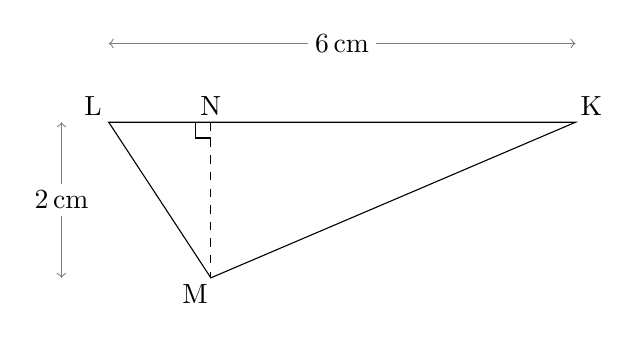
\begin{tikzpicture}[scale=1.0, baseline=(current bounding box.north)]
        \begin{scope}[rotate=180]

        \coordinate (K) at (0,0);
        \coordinate (L) at (5.928,0);
        \coordinate (N) at (4.631,0);
        \coordinate (M) at ($(N)+(0,1.976)$); % Perpendicular upwards

        \draw (K)--(L)--(M)--cycle;
        \draw[dashed] (N)--(M);
        \pic [draw, -, angle radius=0.2cm] {right angle=M--N--L};

        % Vertex LABELS
        % Labels relative to shape geometry
        \node at ($(K)+(-0.2,-0.2)$) {K};
        \node at ($(L)+(0.2,-0.2)$) {L};
        \node at ($(N)+(0.0,-0.2)$) {N};
        \node at ($(M)+(0.2,0.2)$) {M};


        % dotted/dashed arrows shifted away from edges
        % Horizontal side (A-B), shifted down  ift=0mm,
        \draw[<->, gray]
            ($(K) + (0,-1.0cm)$) -- ($(L) + (0,-1.0cm)$)
            node[black, midway, fill=white, inner sep=2.5pt] {6\,cm};

        % Vertical side (B-C), shifted right xshift=0mm,
        \draw[<->, gray]
            ($(L |- N)+(0.6,0)$) -- ($(L |- M)+(0.6,0)$)
            node[black, midway, fill=white, inner sep=2.5pt] {2\,cm};

    \end{scope}
\end{tikzpicture}
\end{minipage}%
\hfill
\begin{minipage}{.4\textwidth}
  \begin{align*}
    \text{Area} &= \frac{1}{2} \text{bh} \\
    \text{Area} &= \frac{1}{2} \times 6 \text{cm} \times 2 \text{cm}  \\
    \text{Area} &= 6.0 \text{cm}^2
  \end{align*}
\end{minipage}

\par\vspace{1cm}\begin{minipage}{0.55\textwidth}
  \refstepcounter{minipagecount}
  \noindent{(\theminipagecount)}\quad
 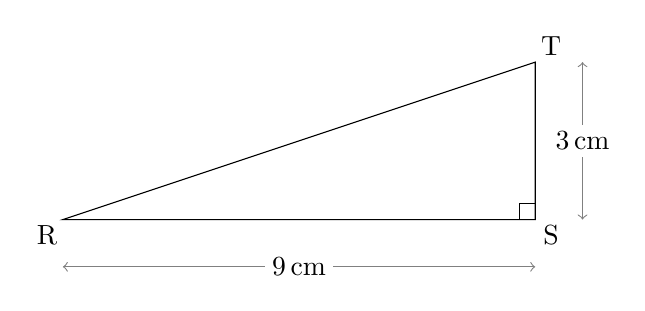
\begin{tikzpicture}[scale=1.0, baseline=(current bounding box.north)]
    \begin{scope}[rotate=0]
        % Draw

        \draw (0,0) coordinate (R) --
         ++(6.0,0) coordinate (S) --
         ++(90:2.0) coordinate (T) -- cycle;

        \pic [draw, -, angle radius=0.2cm] {right angle=T--S--R};

        % Vertex LABELS
        % Labels relative to shape geometry
        \node at ($(R)+(-0.2,-0.2)$) {R};
        \node at ($(S)+(0.2,-0.2)$) {S};
        \node at ($(T)+(0.2,0.2)$) {T};


        % dotted/dashed arrows shifted away from edges
        % Horizontal side (A-B), shifted down
        \draw[<->, gray]
            ($(R) + (0,-0.6cm)$) -- ($(S) + (0,-0.6cm)$)
            node[black, midway, fill=white, inner sep=2.5pt] {9\,cm};

        % Vertical side (B-C), shifted right
        \draw[<->, gray]
            ($(S) + (0.6cm,0)$) -- ($(T) + (0.6cm,0)$)
            node[black, midway, fill=white, xshift=0mm, inner sep=2.5pt] {3\,cm};

    \end{scope}
\end{tikzpicture}
\end{minipage}%
\hfill
\begin{minipage}{.4\textwidth}
  \begin{align*}
    \text{Area} &= \frac{1}{2} \text{bh} \\
    \text{Area} &= \frac{1}{2} \times 9 \text{cm} \times 3 \text{cm}  \\
    \text{Area} &= 13.5 \text{cm}^2
  \end{align*}
\end{minipage}

\par\vspace{1cm}\begin{minipage}{0.55\textwidth}
  \refstepcounter{minipagecount}
  \noindent{(\theminipagecount)}\quad
 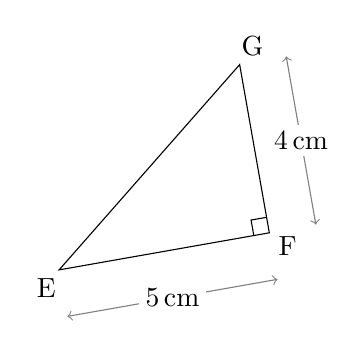
\begin{tikzpicture}[scale=1.0, baseline=(current bounding box.north)]
    \begin{scope}[rotate=10]
        % Draw

        \draw (0,0) coordinate (E) --
         ++(2.711,0) coordinate (F) --
         ++(90:2.169) coordinate (G) -- cycle;

        \pic [draw, -, angle radius=0.2cm] {right angle=G--F--E};

        % Vertex LABELS
        % Labels relative to shape geometry
        \node at ($(E)+(-0.2,-0.2)$) {E};
        \node at ($(F)+(0.2,-0.2)$) {F};
        \node at ($(G)+(0.2,0.2)$) {G};


        % dotted/dashed arrows shifted away from edges
        % Horizontal side (A-B), shifted down
        \draw[<->, gray]
            ($(E) + (0,-0.6cm)$) -- ($(F) + (0,-0.6cm)$)
            node[black, midway, fill=white, inner sep=2.5pt] {5\,cm};

        % Vertical side (B-C), shifted right
        \draw[<->, gray]
            ($(F) + (0.6cm,0)$) -- ($(G) + (0.6cm,0)$)
            node[black, midway, fill=white, xshift=0mm, inner sep=2.5pt] {4\,cm};

    \end{scope}
\end{tikzpicture}
\end{minipage}%
\hfill
\begin{minipage}{.4\textwidth}
  \begin{align*}
    \text{Area} &= \frac{1}{2} \text{bh} \\
    \text{Area} &= \frac{1}{2} \times 5 \text{cm} \times 4 \text{cm}  \\
    \text{Area} &= 10.0 \text{cm}^2
  \end{align*}
\end{minipage}

\par\vspace{1cm}\begin{minipage}{0.55\textwidth}
  \refstepcounter{minipagecount}
  \noindent{(\theminipagecount)}\quad
 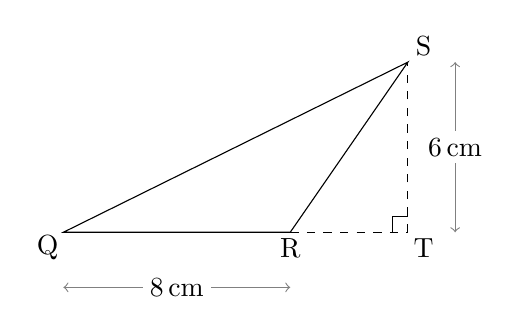
\begin{tikzpicture}[scale=1.0, baseline=(current bounding box.north)]
        \begin{scope}[rotate=0]

        \coordinate (Q) at (0,0);
        \coordinate (R) at (2.881,0);
        \coordinate (T) at ($(R)+(1.494,0)$);  % extend out
        \coordinate (S) at ($(T)+(0,2.161)$); % Perpendicular upwards

        \draw (Q)--(R)--(S)--cycle;
        \draw[dashed] (R)--(T);
        \draw[dashed] (T)--(S);
        \pic [draw, -, angle radius=0.2cm] {right angle=S--T--R};

        % Vertex LABELS
        % Labels relative to shape geometry
        \node at ($(Q)+(-0.2,-0.2)$) {Q};
        \node at ($(R)+(0.0,-0.2)$) {R};
        \node at ($(T)+(0.2,-0.2)$) {T};
        \node at ($(S)+(0.2,0.2)$) {S};


        % dotted/dashed arrows shifted away from edges
        % Horizontal side (A-B), shifted down yshift=0mm,
        \draw[<->, gray]
            ($(Q) + (0,-0.7cm)$) -- ($(R) + (0,-0.7cm)$)
            node[black, midway, fill=white, inner sep=2.5pt] {8\,cm};

        % Vertical side (D-C), shifted right xshift=0mm,
        \draw[<->, gray]
            ($(T)+(0.6,0)$) -- ($(T |- S)+(0.6,0)$)
            node[black, midway, fill=white, inner sep=2.5pt] {6\,cm};
    \end{scope}
\end{tikzpicture}
\end{minipage}%
\hfill
\begin{minipage}{.4\textwidth}
  \begin{align*}
    \text{Area} &= \frac{1}{2} \text{bh} \\
    \text{Area} &= \frac{1}{2} \times 8 \text{cm} \times 6 \text{cm}  \\
    \text{Area} &= 24.0 \text{cm}^2
  \end{align*}
\end{minipage}

\par\vspace{1cm}\begin{minipage}{0.55\textwidth}
  \refstepcounter{minipagecount}
  \noindent{(\theminipagecount)}\quad
 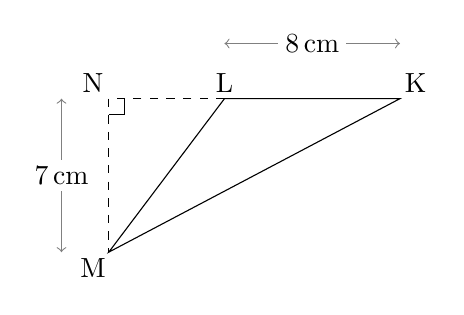
\begin{tikzpicture}[scale=1.0, baseline=(current bounding box.north)]
        \begin{scope}[rotate=180]

        \coordinate (K) at (0,0);
        \coordinate (L) at (2.229,0);
        \coordinate (N) at ($(L)+(1.47,0)$);  % extend out
        \coordinate (M) at ($(N)+(0,1.95)$); % Perpendicular upwards

        \draw (K)--(L)--(M)--cycle;
        \draw[dashed] (L)--(N);
        \draw[dashed] (N)--(M);
        \pic [draw, -, angle radius=0.2cm] {right angle=M--N--L};

        % Vertex LABELS
        % Labels relative to shape geometry
        \node at ($(K)+(-0.2,-0.2)$) {K};
        \node at ($(L)+(0.0,-0.2)$) {L};
        \node at ($(N)+(0.2,-0.2)$) {N};
        \node at ($(M)+(0.2,0.2)$) {M};


        % dotted/dashed arrows shifted away from edges
        % Horizontal side (A-B), shifted down yshift=0mm,
        \draw[<->, gray]
            ($(K) + (0,-0.7cm)$) -- ($(L) + (0,-0.7cm)$)
            node[black, midway, fill=white, inner sep=2.5pt] {8\,cm};

        % Vertical side (D-C), shifted right xshift=0mm,
        \draw[<->, gray]
            ($(N)+(0.6,0)$) -- ($(N |- M)+(0.6,0)$)
            node[black, midway, fill=white, inner sep=2.5pt] {7\,cm};
    \end{scope}
\end{tikzpicture}
\end{minipage}%
\hfill
\begin{minipage}{.4\textwidth}
  \begin{align*}
    \text{Area} &= \frac{1}{2} \text{bh} \\
    \text{Area} &= \frac{1}{2} \times 8 \text{cm} \times 7 \text{cm}  \\
    \text{Area} &= 28.0 \text{cm}^2
  \end{align*}
\end{minipage}

\par\vspace{1cm}\begin{minipage}{0.55\textwidth}
  \refstepcounter{minipagecount}
  \noindent{(\theminipagecount)}\quad
 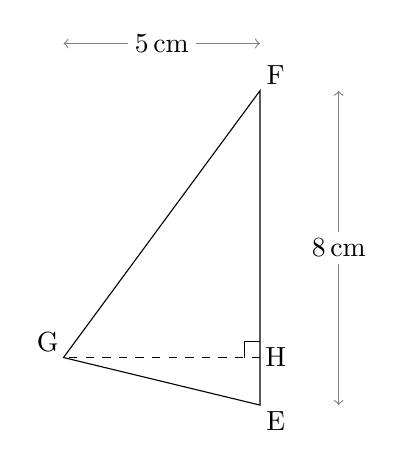
\begin{tikzpicture}[scale=1.0, baseline=(current bounding box.north)]
        \begin{scope}[rotate=90]

        \coordinate (E) at (0,0);
        \coordinate (F) at (3.992,0);
        \coordinate (H) at (0.604,0);
        \coordinate (G) at ($(H)+(0,2.495)$); % Perpendicular upwards

        \draw (E)--(F)--(G)--cycle;
        \draw[dashed] (H)--(G);
        \pic [draw, -, angle radius=0.2cm] {right angle=G--H--F};

        % Vertex LABELS
        % Labels relative to shape geometry
        \node at ($(E)+(-0.2,-0.2)$) {E};
        \node at ($(F)+(0.2,-0.2)$) {F};
        \node at ($(H)+(0.0,-0.2)$) {H};
        \node at ($(G)+(0.2,0.2)$) {G};


        % dotted/dashed arrows shifted away from edges
        % Horizontal side (A-B), shifted down  ift=0mm,
        \draw[<->, gray]
            ($(E) + (0,-1.0cm)$) -- ($(F) + (0,-1.0cm)$)
            node[black, midway, fill=white, inner sep=2.5pt] {8\,cm};

        % Vertical side (B-C), shifted right xshift=0mm,
        \draw[<->, gray]
            ($(F |- H)+(0.6,0)$) -- ($(F |- G)+(0.6,0)$)
            node[black, midway, fill=white, inner sep=2.5pt] {5\,cm};

    \end{scope}
\end{tikzpicture}
\end{minipage}%
\hfill
\begin{minipage}{.4\textwidth}
  \begin{align*}
    \text{Area} &= \frac{1}{2} \text{bh} \\
    \text{Area} &= \frac{1}{2} \times 8 \text{cm} \times 5 \text{cm}  \\
    \text{Area} &= 20.0 \text{cm}^2
  \end{align*}
\end{minipage}

\par\vspace{1cm}\begin{minipage}{0.55\textwidth}
  \refstepcounter{minipagecount}
  \noindent{(\theminipagecount)}\quad
 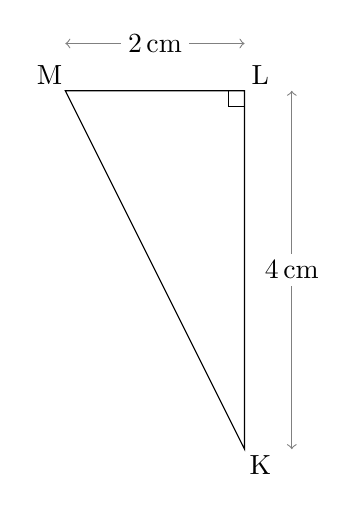
\begin{tikzpicture}[scale=1.0, baseline=(current bounding box.north)]
    \begin{scope}[rotate=90]
        % Draw

        \draw (0,0) coordinate (K) --
         ++(4.552,0) coordinate (L) --
         ++(90:2.276) coordinate (M) -- cycle;

        \pic [draw, -, angle radius=0.2cm] {right angle=M--L--K};

        % Vertex LABELS
        % Labels relative to shape geometry
        \node at ($(K)+(-0.2,-0.2)$) {K};
        \node at ($(L)+(0.2,-0.2)$) {L};
        \node at ($(M)+(0.2,0.2)$) {M};


        % dotted/dashed arrows shifted away from edges
        % Horizontal side (A-B), shifted down
        \draw[<->, gray]
            ($(K) + (0,-0.6cm)$) -- ($(L) + (0,-0.6cm)$)
            node[black, midway, fill=white, inner sep=2.5pt] {4\,cm};

        % Vertical side (B-C), shifted right
        \draw[<->, gray]
            ($(L) + (0.6cm,0)$) -- ($(M) + (0.6cm,0)$)
            node[black, midway, fill=white, xshift=0mm, inner sep=2.5pt] {2\,cm};

    \end{scope}
\end{tikzpicture}
\end{minipage}%
\hfill
\begin{minipage}{.4\textwidth}
  \begin{align*}
    \text{Area} &= \frac{1}{2} \text{bh} \\
    \text{Area} &= \frac{1}{2} \times 4 \text{cm} \times 2 \text{cm}  \\
    \text{Area} &= 4.0 \text{cm}^2
  \end{align*}
\end{minipage}

\par\vspace{1cm}

\end{document}
